% Homework template for Inference and Information
% UPDATE: September 26, 2017 by Xiangxiang
\documentclass[a4paper]{article}
\usepackage{ctex}
\usepackage{amsmath, amssymb, amsthm}
\usepackage{moreenum}
\usepackage{mathtools}
\usepackage{url}
\usepackage{bm}
\usepackage{enumitem}
\usepackage{graphicx}
\usepackage{listings}
\usepackage{color}

\usepackage{fontspec}
\usepackage{xcolor}

\usepackage{float}

\definecolor{codekeyword}{RGB}{171, 0, 216}
\definecolor{codetypename}{RGB}{29, 37, 251}
\definecolor{codevariable}{RGB}{10, 23, 126}
\definecolor{codestring}{RGB}{157, 0, 25}
\definecolor{codecomment}{RGB}{31, 129, 19}
\definecolor{codebackground}{RGB}{230 235 245}

\newfontfamily\cascadia[Ligatures=ResetAll]{Cascadia Code}

\lstset{
    basicstyle          =   \footnotesize\cascadia,          % 基本代码风格
    keywordstyle        =   \bfseries,          % 关键字风格
    commentstyle        =   \rmfamily\itshape,  % 注释的风格,斜体
    stringstyle         =   \ttfamily,  % 字符串风格
    flexiblecolumns,                % 别问为什么,加上这个
    numbers             =   left,   % 行号的位置在左边
    showspaces          =   false,  % 是否显示空格,显示了有点乱,所以不现实了
    numberstyle         =   \cascadia,    % 行号的样式,小五号,tt等宽字体
    showstringspaces    =   false,
    captionpos          =   t,      % 这段代码的名字所呈现的位置,t指的是top上面
    backgroundcolor     =   \color{codebackground},
    breaklines          =   true,
    frame               =   l,
}

\lstdefinestyle{Python}{
    language        =   Python, % 语言选Python
    basicstyle      =   \zihao{-5}\ttfamily,
    numberstyle     =   \zihao{-5}\ttfamily,
    keywordstyle    =   \color{blue},
    keywordstyle    =   [2] \color{teal},
    stringstyle     =   \color{magenta},
    commentstyle    =   \color{red}\ttfamily,
    breaklines      =   true,   % 自动换行,建议不要写太长的行
    columns         =   fixed,  % 如果不加这一句,字间距就不固定,很丑,必须加
    basewidth       =   0.5em,
}
\usepackage{subcaption}
\usepackage{booktabs} % toprule
\usepackage[mathcal]{eucal}
\usepackage[thehwcnt = 2]{iidef}

\setenumerate[1]{label=(\arabic{*})}
\setenumerate[2]{label=\arabic{*})}



\thecourseinstitute{清华大学电子工程系}
\thecoursename{\textbf{媒体与认知} \space 课堂2}
\theterm{2023-2024学年春季学期}
\hwname{作业}
\begin{document}
\courseheader
\name{毕嘉仪}
\vspace{3mm}
\centerline{\textbf{\Large{理论部分}}}

\section{单选题(15分)}
\subsection{\underline{C}}

\subsection{\underline{D}}

\subsection{\underline{D}}

\subsection{\underline{C}}

\subsection{\underline{B}}

\section{计算题(15 分)}
\subsection{
已知某卷积层的输入为$X$(该批量中样本数目为1,输入样本通道数为1),采用一个卷积核$W$,即卷积输出通道数为1,卷积核尺寸为$2\times 2$,卷积的步长为1,无边界延拓,偏置量为$b$:
$$X=\left[ \begin{array}{ccc}
    0.5 & -0.2 & 0.3 \\
    0.6 & 0.4 & -0.1 \\
    -0.4 & 0.5 & 0.2
\end{array}\right],
W=\left[ \begin{array}{cc}
    0.1 & -0.2  \\
    -0.3 & 0.4
\end{array}\right], b=0.04$$
}
\subsubsection{请计算卷积层的输出$Y$。}

\[y_{11} = 0.05 + 0.04 - 0.18 + 0.16 + 0.04 = 0.11\]
\[y_{12} = -0.02 - 0.02 - 0.12 - 0.04 + 0.04 = -0.20\]
\[y_{21} = 0.06 - 0.08 + 0.12 + 0.20 + 0.04 = 0.34\]
\[y_{22} = 0.04 + 0.02 - 0.15 + 0.08 + 0.04 = 0.03\]
\[\therefore Y = \begin{bmatrix}
                0.11 & -0.20 \\
                0.34 & 0.03 \\
                \end{bmatrix}\]

\subsubsection{若训练过程中的目标函数为$L$,且已知$\frac{\partial L}{\partial Y}=\left[ \begin{array}{cc}
    0.3 & 0.1 \\
    -0.4 & 0.2
\end{array} \right]$,请计算$\frac{\partial L}{\partial X}$。
}
\begin{align*}
    \frac{\partial L}{\partial X} &= \mathrm{zero\_padded}(Y) * W^{\mathrm{T}} \\
    &= \begin{bmatrix}
        0 & 0 & 0 & 0 \\
        0 & 0.11 & -0.20 & 0 \\
        0 & 0.34 & 0.03 & 0 \\
        0 & 0 & 0 & 0 \\
    \end{bmatrix} *
    \begin{bmatrix}
        0.4 & -0.3 \\
        -0.2 & 0.1 \\
    \end{bmatrix} \\
    &= \begin{bmatrix}
        0.011 & 0.104 & 0.004 \\
        0.001 & 0.039 & -0.086 \\
        -0.102 & 0.127 &0.012 \\
    \end{bmatrix}
\end{align*}

注:本题的计算方式不限,但需要提供计算过程以及各步骤的结果。
\vspace{6mm}

\centerline{\textbf{\Large{编程部分}}}
\vspace{3mm}

% 请根据是否选择自选课题的情况选择“编程作业报告”或“自选课题开题报告”中的一项完成
\section{编程作业报告}
\begin{enumerate}
    \item 探究 batch normalization 和 dropout 的作用
    
    \begin{enumerate}
        \item 使用默认配置(不启用 BN 和 dropout),训练 baseline 模型:
        
        经过多次试验与测试,发现默认参数配置下的模型效果就已经是最好的了。

        训练模型:
        
        input:
        \lstinputlisting{../result/1_1_in_train-0.txt}

        output:
        \lstinputlisting{../result/1_1_out_train-0.txt}
        \begin{figure}[H]
            \centering
            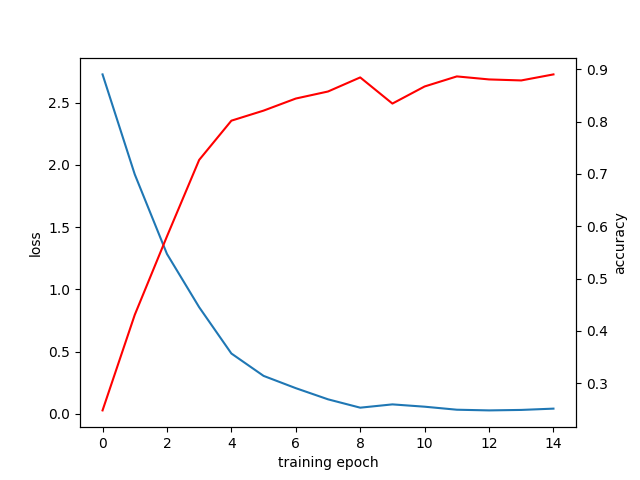
\includegraphics[width=0.65\linewidth]{../result/1_1-0.png}
            \caption{}
        \end{figure}

        测试模型:

        input:
        \lstinputlisting{../result/1_1_in_test-0.txt}

        output:
        \lstinputlisting{../result/1_1_out_test-0.txt}
        \vspace{2em}

        \item 启用 batch normalization:
        
        经过多次试验与测试,发现默认参数配置下的模型效果就已经是最好的了。

        训练模型:

        input:
        \lstinputlisting{../result/1_2_in_train-0.txt}

        output:
        \lstinputlisting{../result/1_2_out_train-0.txt}
        \begin{figure}[H]
            \centering
            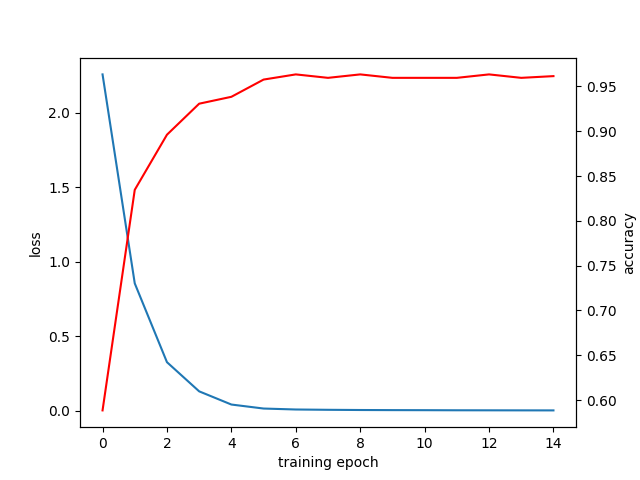
\includegraphics[width=0.65\linewidth]{../result/1_2-0.png}
            \caption{}
        \end{figure}

        测试模型:

        input:
        \lstinputlisting{../result/1_2_in_test-0.txt}

        output:
        \lstinputlisting{../result/1_2_out_test-0.txt}

        分析:测试准确率明显提升,收敛速度也大大加快。
        \vspace{2em}

        \item 启用 dropout 并设置概率为 0.3:
        训练模型:

        input:
        \lstinputlisting{../result/1_3_in_train-0.txt}

        output:
        \lstinputlisting{../result/1_3_out_train-0.txt}
        \begin{figure}[H]
            \centering
            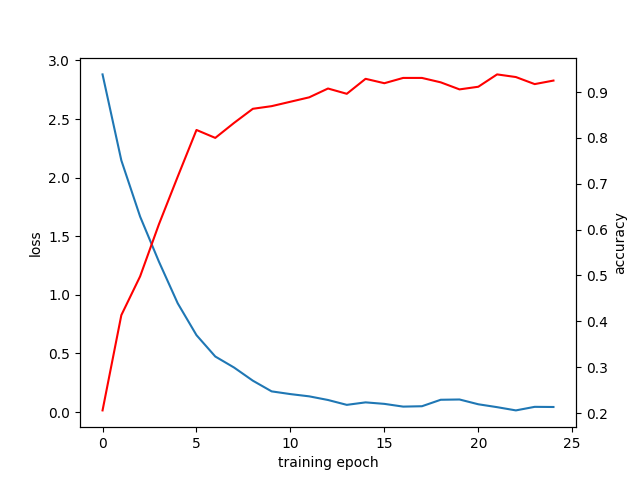
\includegraphics[width=0.65\linewidth]{../result/1_3-25epoch.png}
            \caption{}
        \end{figure}

        测试模型:

        input:
        \lstinputlisting{../result/1_3_in_test-0.txt}

        output:
        \lstinputlisting{../result/1_3_out_test-0.txt}

        分析:测试准确率明显提升,收敛速度有所降低。

    \end{enumerate}
    \vspace{2em}


    \item 探究数据增广的作用
    \begin{enumerate}
        \item 数据增广变换
        input:
        \lstinputlisting{../result/2_1_in.txt}

        output:
        \lstinputlisting{../result/2_1_out.txt}
        \begin{figure}[H]
            \centering
            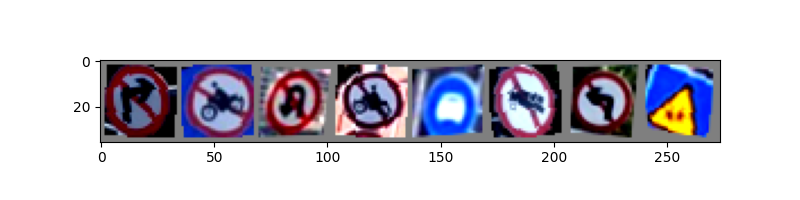
\includegraphics[width=\linewidth]{../result/2_1.png}
            \caption{}
        \end{figure}

        其中,所使用的增广变换为
        \begin{lstlisting}[style=Python]
if mode == "train" and augment:
    data_transforms.append(transforms.RandomRotation(10))
    data_transforms.append(transforms.RandomPerspective(0.2))
        \end{lstlisting}

        选择原因:首先,数据图像已将路牌主体呈现在画面中央,因此random crop效果并不会好;其次,由于拍摄角度问题,路牌图像的旋转角度和透视效果不一,因此选择这两种transform可以实现比较合理的数据增广。
        \vspace{2em}

        \item 模型训练与测试
        训练模型:

        input:
        \lstinputlisting{../result/2_2_in_train.txt}

        output:
        \lstinputlisting{../result/2_2_out_train.txt}
        \begin{figure}[H]
            \centering
            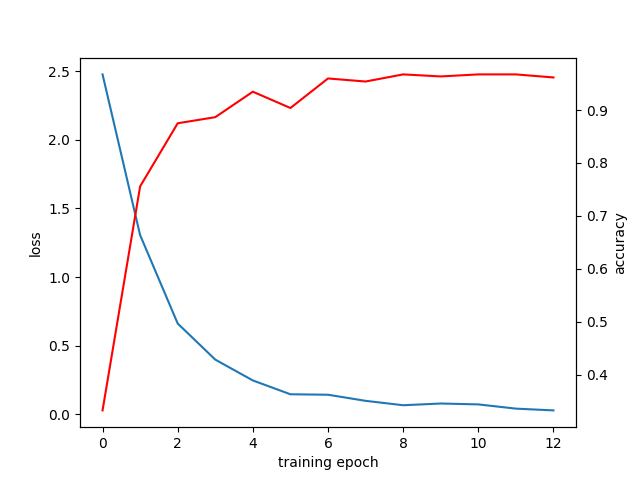
\includegraphics[width=0.65\linewidth]{../result/2_2.png}
            \caption{}
        \end{figure}

        测试模型:

        input:
        \lstinputlisting{../result/2_2_in_test.txt}

        output:
        \lstinputlisting{../result/2_2_out_test.txt}


    \end{enumerate}
    \vspace{2em}


    \item 探究空间变换网络 (STN) 的作用
    
    \vspace{2em}


    \item 可视化
    \begin{enumerate}
        \item[]
        分别输入以下命令:
        \lstinputlisting{../result/4_in.txt}
        \vspace{2em}

        \item 可视化各卷积层的卷积核:
        \begin{figure}[H]
            \centering
            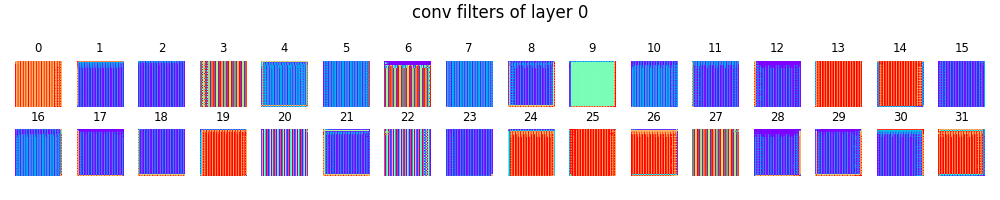
\includegraphics[width=0.65\linewidth]{../result/4_conv_filters_layer0.png}
            \caption{}
        \end{figure}
        \begin{figure}[H]
            \centering
            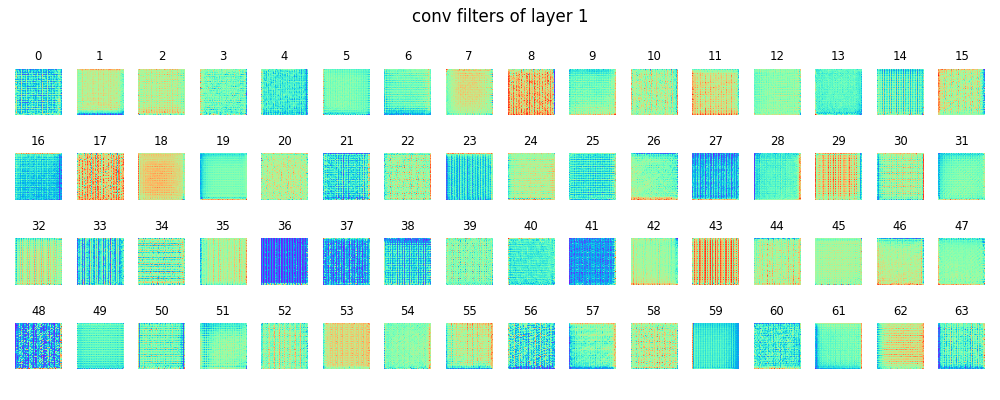
\includegraphics[width=0.65\linewidth]{../result/4_filter_layer1.png}
            \caption{}
        \end{figure}
        \begin{figure}[H]
            \centering
            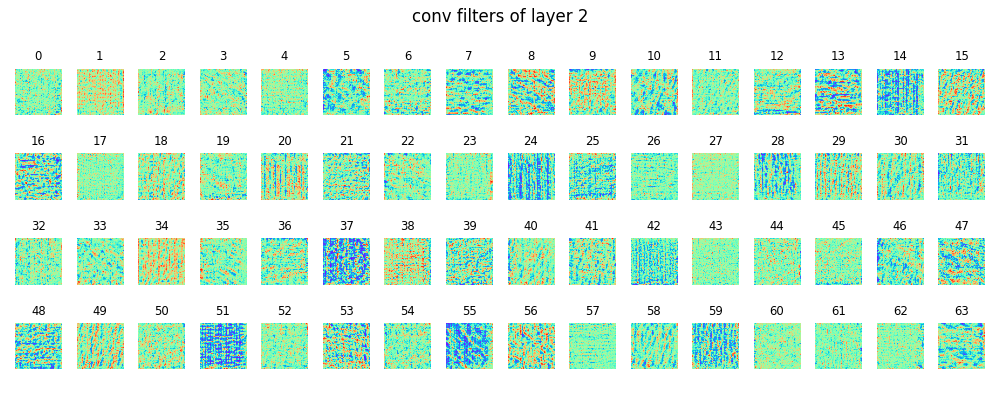
\includegraphics[width=0.65\linewidth]{../result/4_filter_layer2.png}
            \caption{}
        \end{figure}
        \begin{figure}[H]
            \centering
            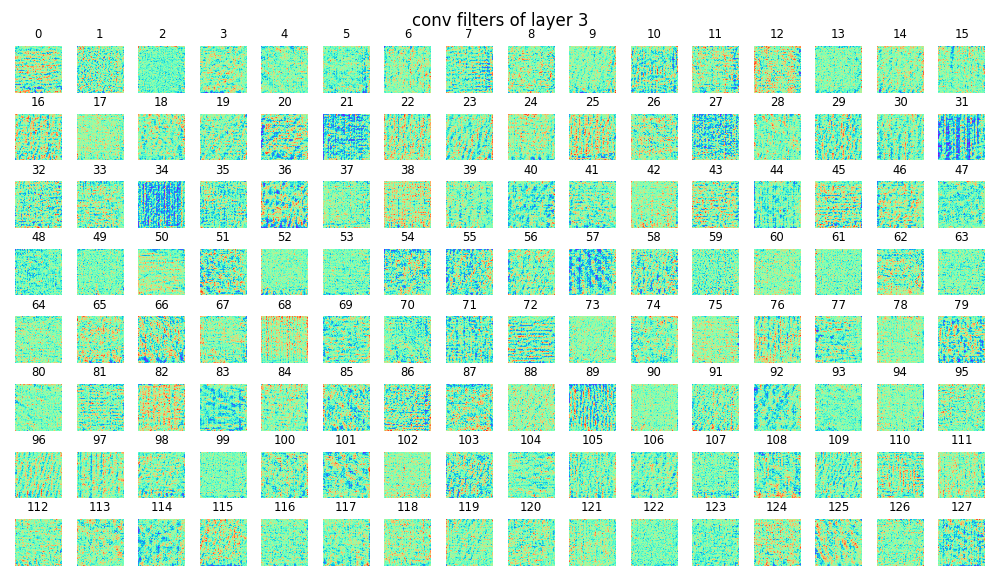
\includegraphics[width=0.65\linewidth]{../result/4_filter_layer3.png}
            \caption{}
        \end{figure}
        \begin{figure}[H]
            \centering
            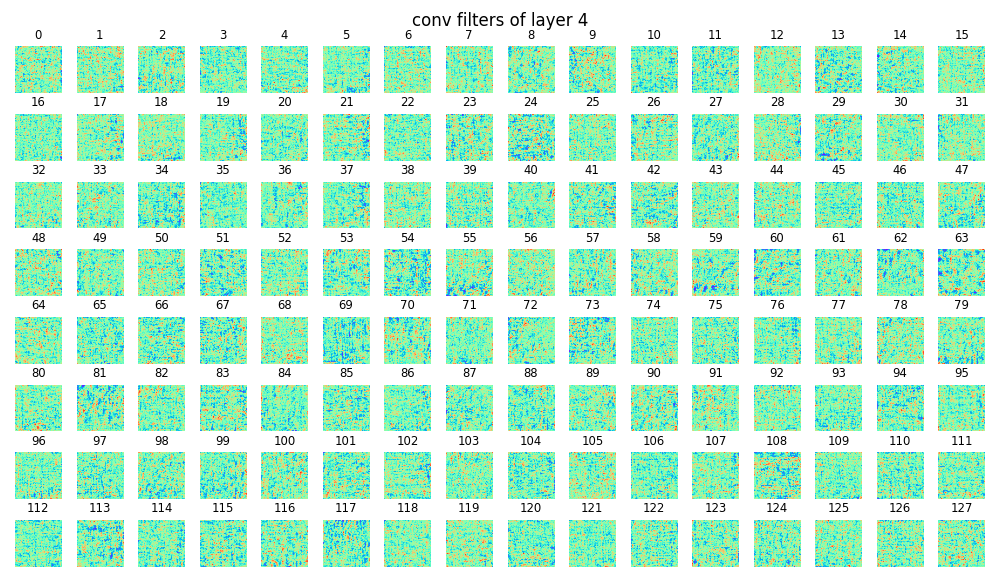
\includegraphics[width=0.65\linewidth]{../result/4_filter_layer4.png}
            \caption{}
        \end{figure}

        \item 可视化第50张图像个卷积层的输出特征图:
        \begin{figure}[H]
            \centering
            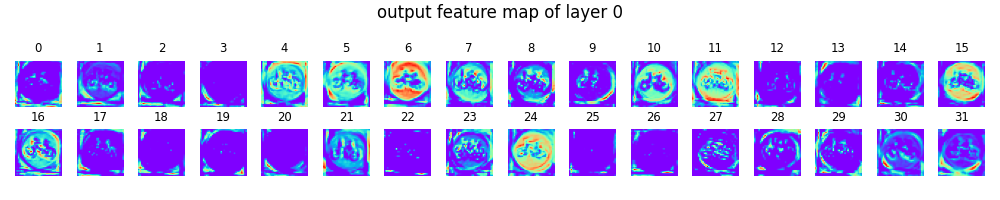
\includegraphics[width=0.65\linewidth]{../result/4_feature_layer0.png}
            \caption{}
        \end{figure}
        \begin{figure}[H]
            \centering
            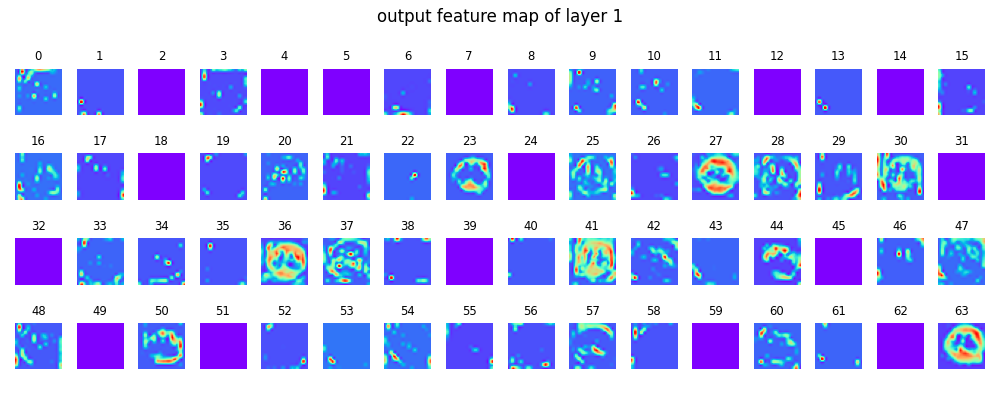
\includegraphics[width=0.65\linewidth]{../result/4_feature_layer1.png}
            \caption{}
        \end{figure}
        \begin{figure}[H]
            \centering
            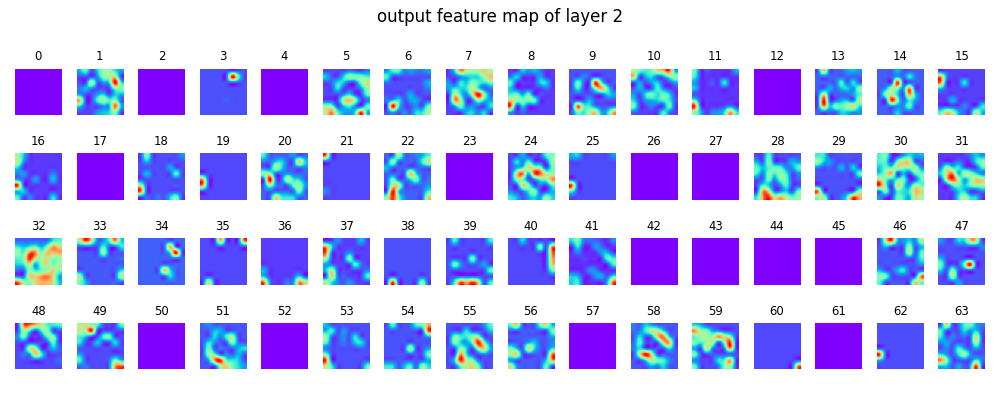
\includegraphics[width=0.65\linewidth]{../result/4_feature_layer2.png}
            \caption{}
        \end{figure}
        \begin{figure}[H]
            \centering
            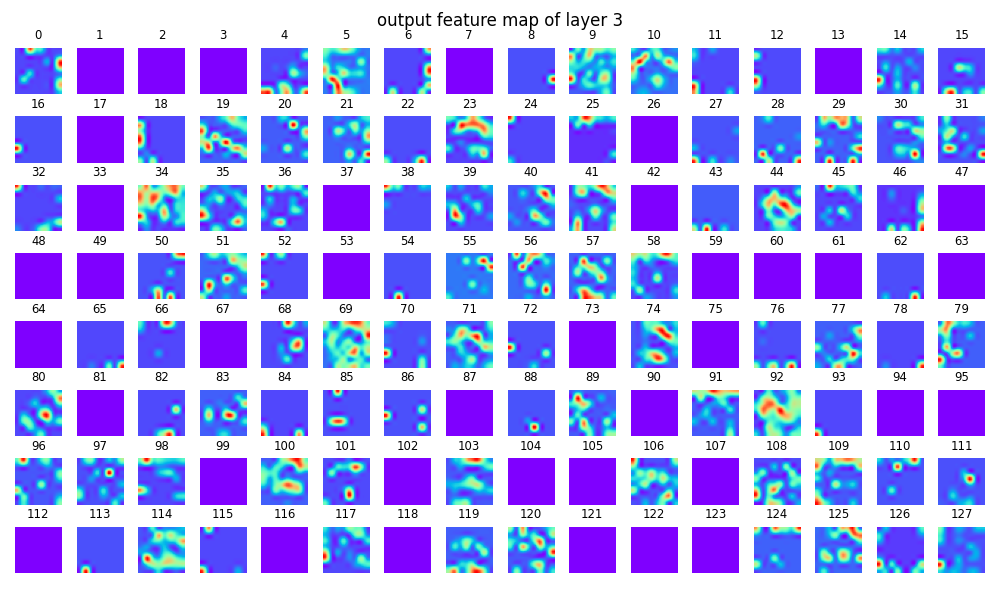
\includegraphics[width=0.65\linewidth]{../result/4_feature_layer3.png}
            \caption{}
        \end{figure}
        \begin{figure}[H]
            \centering
            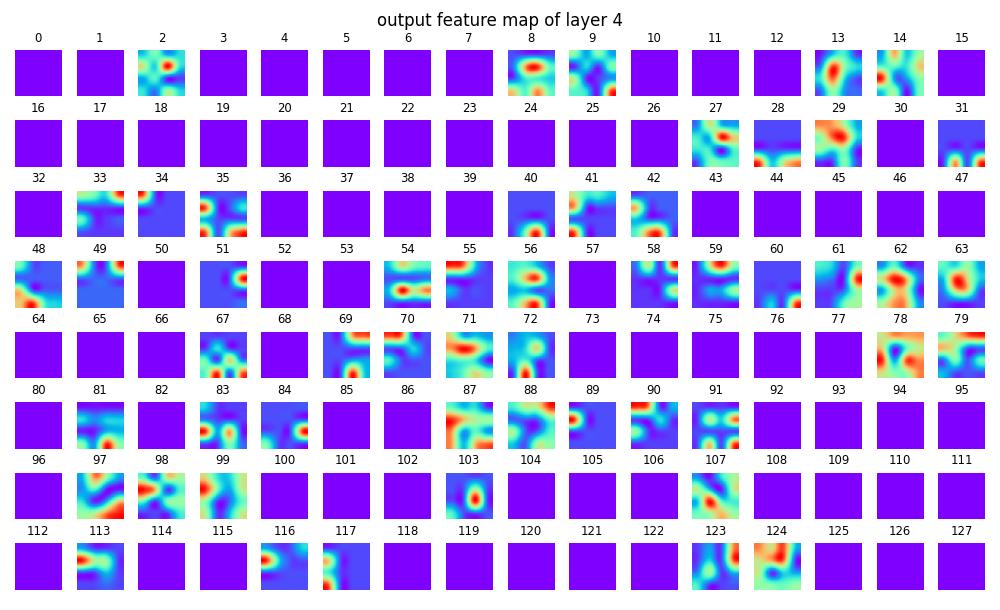
\includegraphics[width=0.65\linewidth]{../result/4_feature_layer4.png}
            \caption{}
        \end{figure}
        可见,随着卷积层数的增加,图像的不同特征不断被提取、分离、放大,在最后一张特征图中最为鲜明。
        \vspace{2em}

        \item  t-SNE 可视化最后一层隐藏层的输出特征:
        \begin{figure}[H]
            \centering
            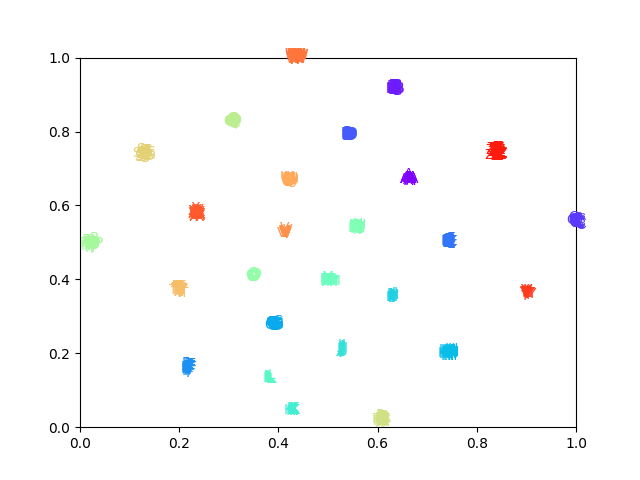
\includegraphics[width=0.65\linewidth]{../result/4_tsne.png}
            \caption{}
        \end{figure}
        可见,各个类型的标牌被明确地分成了不同类别。
        \vspace{2em}

        \item 可视化 STN 学习到的变换:
        \begin{figure}[H]
            \centering
            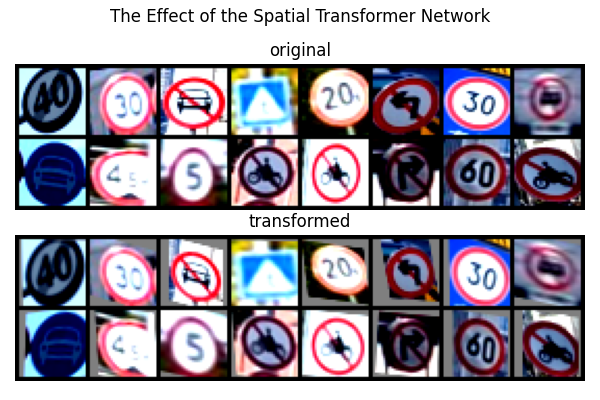
\includegraphics[width=0.65\linewidth]{../result/4_stn.png}
            \caption{}
        \end{figure}

    \end{enumerate}

    


\end{enumerate}


\section{遇到的问题及解决方法}
    \begin{enumerate}
        \item 
    \end{enumerate}

\section{建议}



\end{document}



%%% Local Variables:
%%% mode: late\rvx
%%% TeX-master: t
%%% End:
